%!TEX root = ../../../main.tex




\section[g2 Measurements]{Photon correlation measurements} \label{sec::g2}



	\begin{figure}[tp]
		\begin{subfigure}[tp]{ 0.49\linewidth}
			\caption{}\label{subfig::g2_a}
			\centering
			\testbox{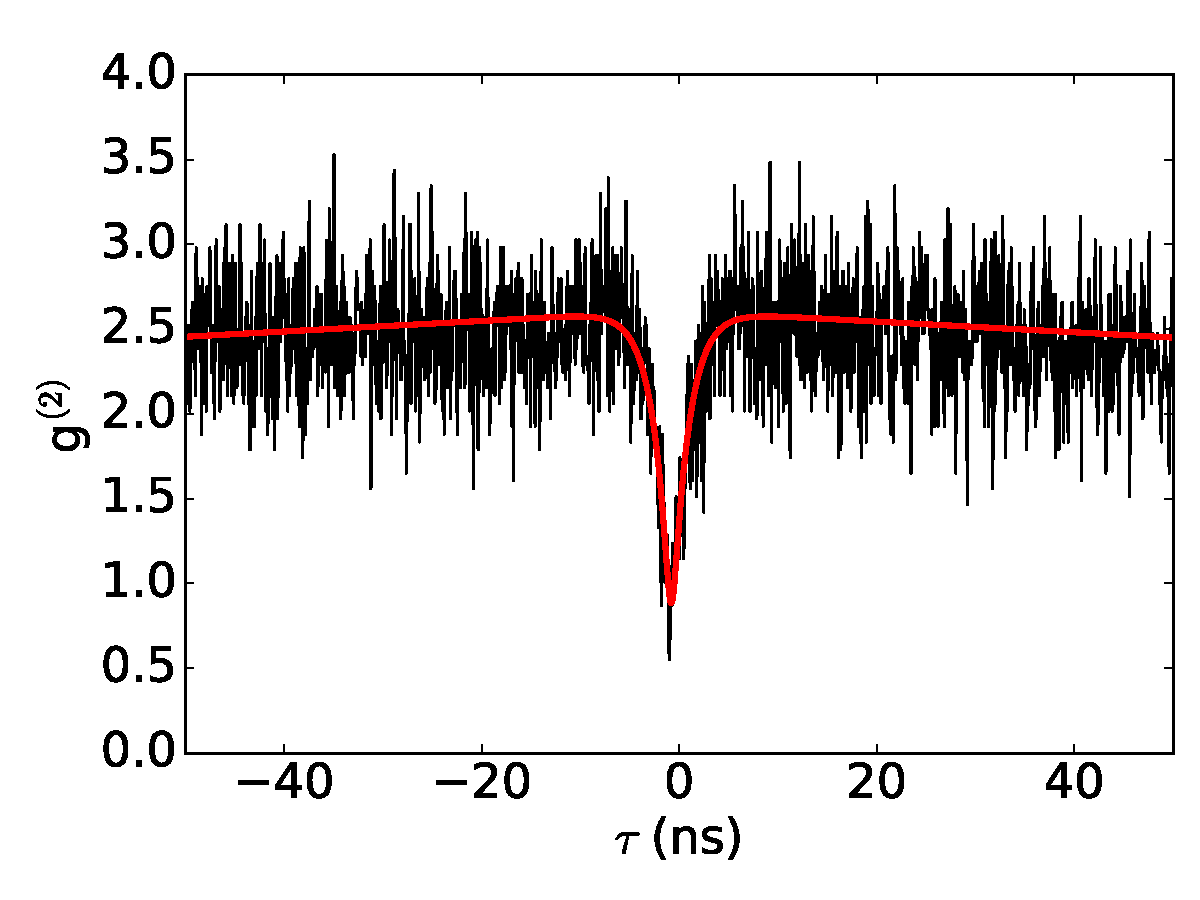
\includegraphics[trim = 0 0 0 0,  clip= true, width = \textwidth]{./pics/Ir8_g2zuSpektrum8_15_5_corr_fit_notitle.pdf}}
		\end{subfigure}
		\hfill
		\begin{subfigure}[tp]{ 0.49\linewidth}
			\caption{}\label{subfig::g2_b}
			\centering
			\testbox{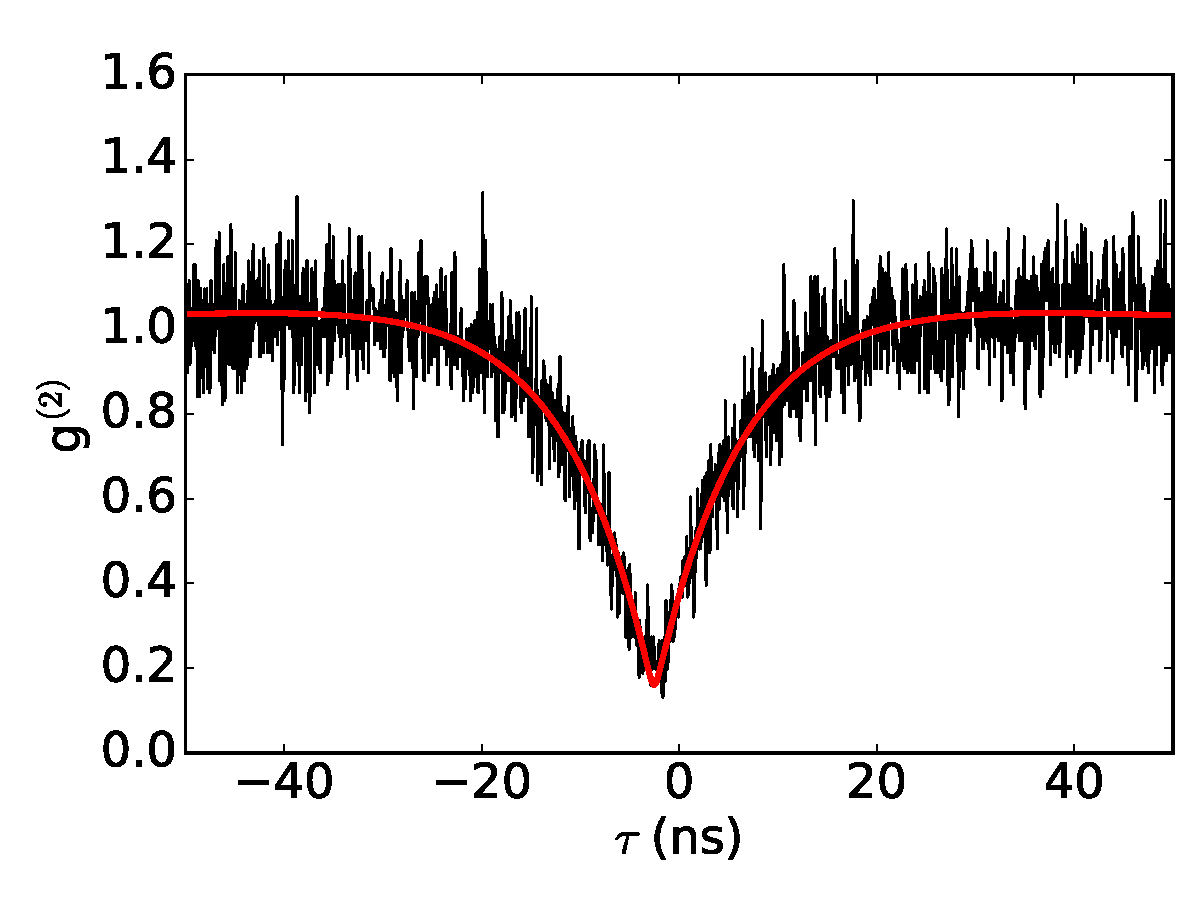
\includegraphics[trim = 0 0 0 0,  clip= true, width = \textwidth]{./pics/Ir8_g2_scan_xy-05_200uW_fit.pdf}}
		\end{subfigure}
		\caption{(a) Intensity autocorrelation function of \emnarrow at an excitation power of \SI{15}{\micro\W}. (b) Intensity autocorrelation function of \embroad at an excitation power of \SIlist{200}{\micro\W}, which is 25\% of the saturation count rate.}
		\label{fig::g2}
	\end{figure}


	The investigated \sivs exhibit count rates of a few thousand to a few \SI{100000}{cps}.
	We carried out measurements of the photon statistics and found that about 3\% of the \sivs are single color centers.
	These measurements show, that the probability of finding a single emitter does not correlate in any way with the \cwl of the ZPL or the \lw of the ZPL.
	We found several single \sivs with an antibunching dip down to about \num{0.2} and attribute the residual \gtz value to background fluorescence from the diamond host.
	For the utilized \nds an of the background measurement independent of \siv \pl is impossible, because the laser spot size is bigger than the \nd. 
	Therefore, the \siv will always be excited when the \nd is illuminated.
	The measured lifetimes of the single \sivs are in the range of \SIrange{1}{7}{ns}.
	\autoref{fig::g2} shows the \gt functions of the two emitters introduced in \autoref{subsec::spectra}, \emnarrow and \embroad.
	\\
	\autoref{subfig::g2_a} shows the photon correlation function of \emnarrow at a power of \SI{15}{\micro\W}. 
	The fit of the data for an excitation power of \SI{15}{\micro\W} yields a lifetime of the excited state of \SI[separate-uncertainty]{1.6\pm0.1}{ns}.
	The \gtz values of the same fit is \num{0.88}, which corresponds to eight equally bright emitters.
	However, the \gtz value is probably overestimated due to the fast dynamics of the emitter which cannot be fully resolved.
	Measurements of other \sivs in \hl yield \gtz values down to \num[separate-uncertainty]{0.2}.
	\\
	\autoref{subfig::g2_b} shows the \gt function of \embroad at an excitation power of \SI{200}{\micro\W}, which is 25\% of the saturation power of that emitter, which amounts to \SI{1}{mW}.
	The \gtz values for yields \num[separate-uncertainty]{0.16\pm0.06}, therefore being a representative \gt measurement of single \sivs.
	The fits yield a lifetime of the excited state of \SI[separate-uncertainty]{6.3\pm0.2}{ns}.
	While it is not 0, it is well below \num{0.5}, indicating single photon emission.
	The non-vanishing \gtz value is caused by background fluorescence of the diamond.
	\\
	Several spectra contain multiple narrow distinct peaks at different \ZPL \cwls.
	This circumstance is attributed to a \nd containing more than one \siv, each of which is subject to a different \cwl shift.
	We choose narrow bandpass filters to perform independent measurements of each individual \siv peak of such a spectrum.
	Therefore it is possible to measure \gtz values below \num{0.5} for each of those narrow peaks.
	Hence the individual peaks are identified as single emitters with a different ZPL \cwl.
	\\
	\begin{figure}[tp]

	\end{figure}

	\begin{figure}[t]
		\begin{subfigure}[t]{ 0.49\linewidth}
			\centering
			\caption{}
			\testbox{\includegraphics[trim = 0 0 0 0,  clip= true, width = \textwidth]{./pics/Ir8_g2_scan_xy-05_100ns_notitle.pdf}}
		\label{fig::g2_powerdependent}
		\end{subfigure}
		\hfill
		\begin{subfigure}[t]{ 0.49\linewidth}
			\centering
			\caption{}
			\testbox{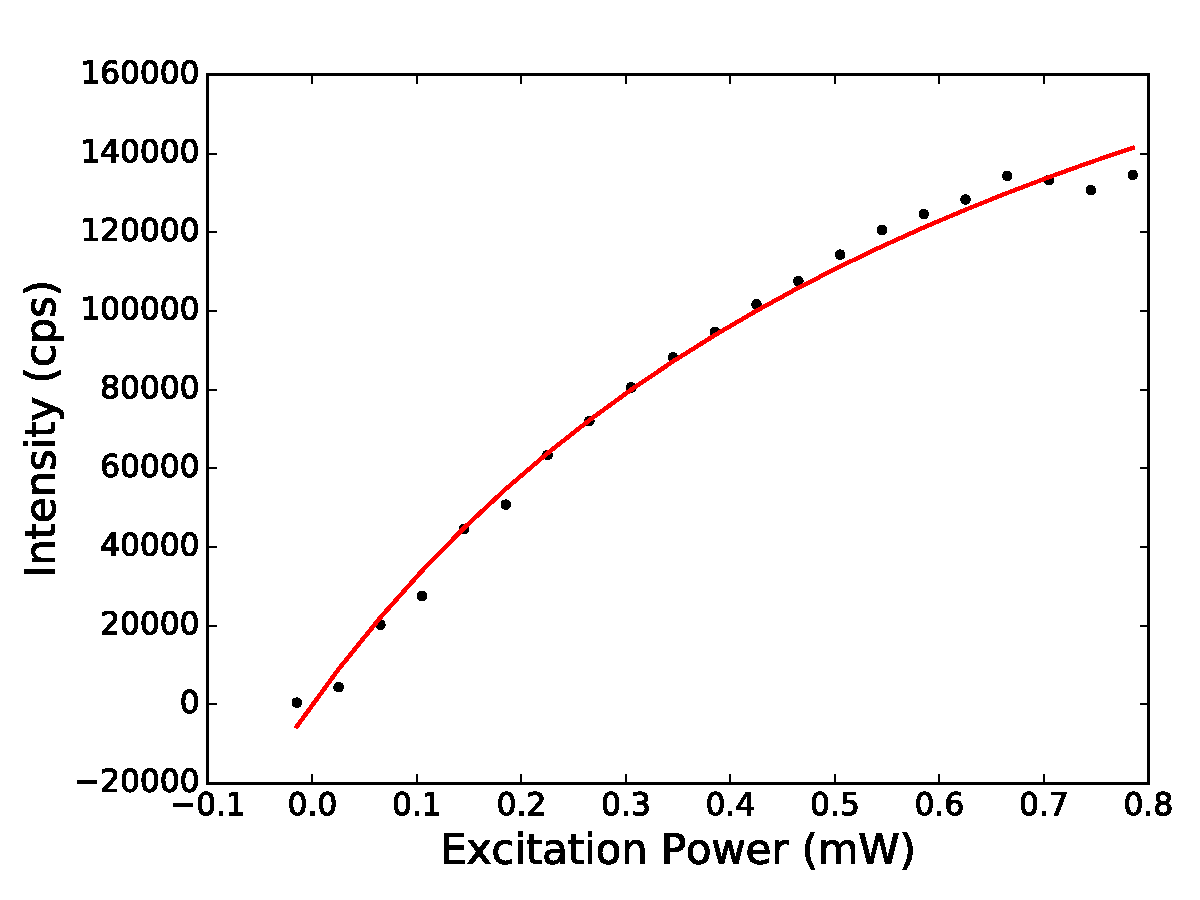
\includegraphics[trim = 0 0 0 0,  clip= true, width = \textwidth]{./pics/Ir8_sat_scan_xy-05_fit_notitle.pdf}}
			\label{subfig::sat_Ir8}
		\end{subfigure}
		\caption{a) The \gtf of emitter xx at an excitation power of \SIlist{200;400;500}{\micro\watt} from bottom to top. b) Saturation measurement of the same emitter.}
		\label{fig::<fig>}
	\end{figure}

	\begin{figure}[tp]
		\begin{subfigure}[t]{ 0.49\linewidth}
			\centering
			\caption{}
			\testbox{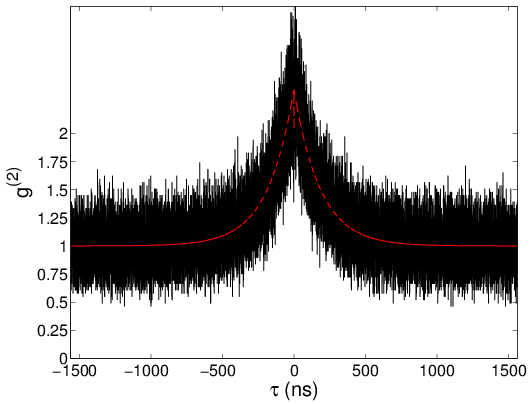
\includegraphics[trim = 0 0 0 0,  clip= true, width = \textwidth]{./pics/Ir22_g2_scan_xy01_x26y25_2V.png}}
			\label{subfig::g2_fast_detail}
		\end{subfigure}
		\hfill
		\begin{subfigure}[t]{ 0.49\linewidth}
			\centering
			\caption{}
			\testbox{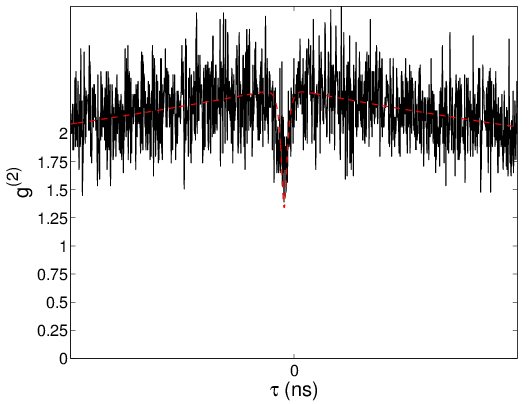
\includegraphics[trim = 0 0 0 0,  clip= true, width = \textwidth]{./pics/Ir22_g2_scan_xy01_x26y25_2V_g2_normalized_middle50ns.png}}
			\label{subfig::g2_fast_all}
		\end{subfigure}
		\caption{Photon autocorrelation measurement of emitter \correct{xx} at an excitation power of \SI{500}{\micro\watt}. a) It is evident, that is exhibits a strong bunching. b) In a detail image a small antibunching dip can be seen. While it can be fit with the fitting function of a single emitter, the dip probably does not get fully resolved due to fast dynamics.}
		\label{fig::g2_fast}

	\end{figure}
	\todo{think of emitter names}
	Due to fast dynamics of the SiV center and the limited timing resolution of the APDs in the experimental setup (overall resolution of  \textasciitilde{}\SI{700}{ps}) it is not possible to fully resolve the narrow antibunching dip down to lower g(2)(0) values. The fit yields a lifetime of the excited state of \SI{710\pm30}{ps} at an excitation power of \SI{500}{\micro\watt}.
	\\
	\begin{figure}[tp]
		\begin{subfigure}[t]{ 0.49\linewidth}
			\centering
			\caption{}
			\testbox{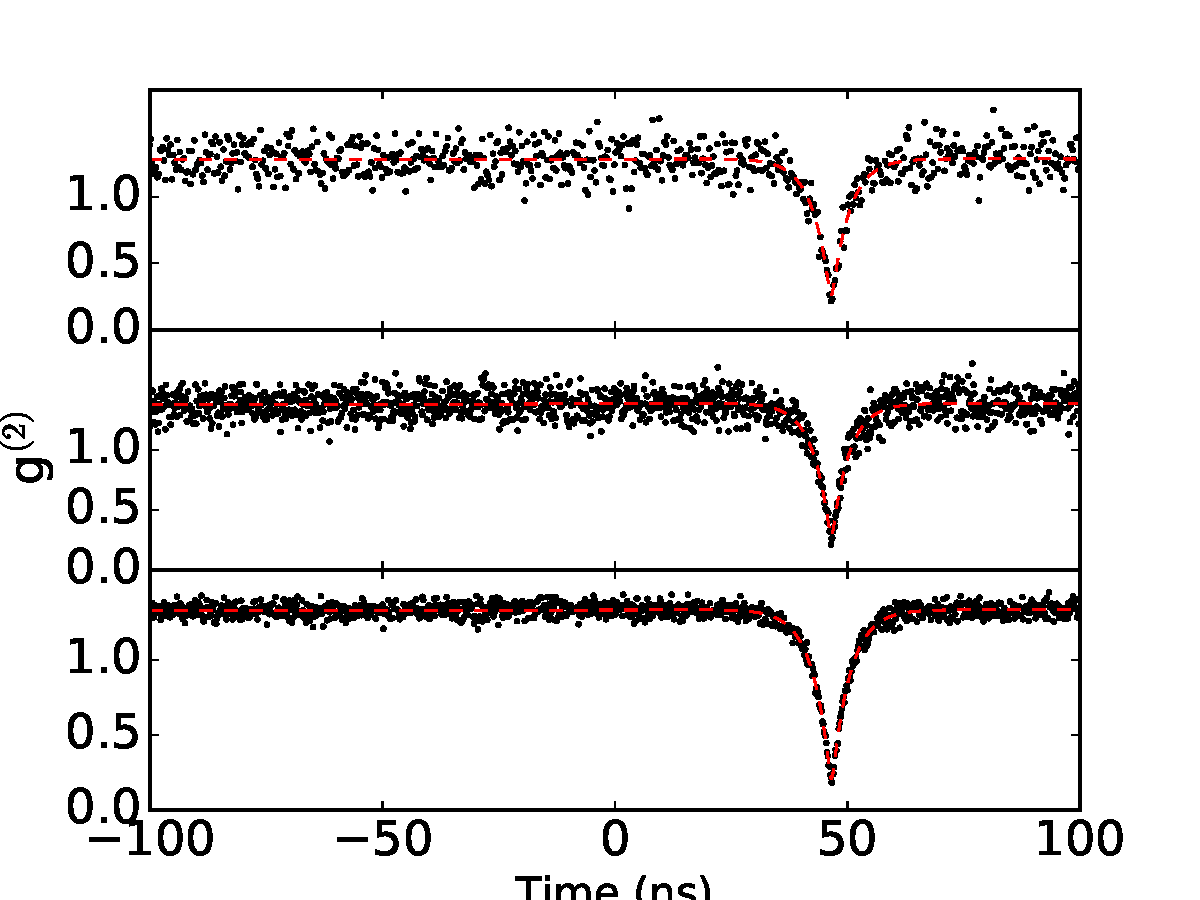
\includegraphics[trim = 0 0 0 0,  clip= true, width = \textwidth]{./pics/erlangen_g2_all.pdf}}
			\label{subfig::erlangen_g2_all}
		\end{subfigure}
		\hfill
		\begin{subfigure}[t]{ 0.49\linewidth}
			\centering
			\caption{}
			\testbox{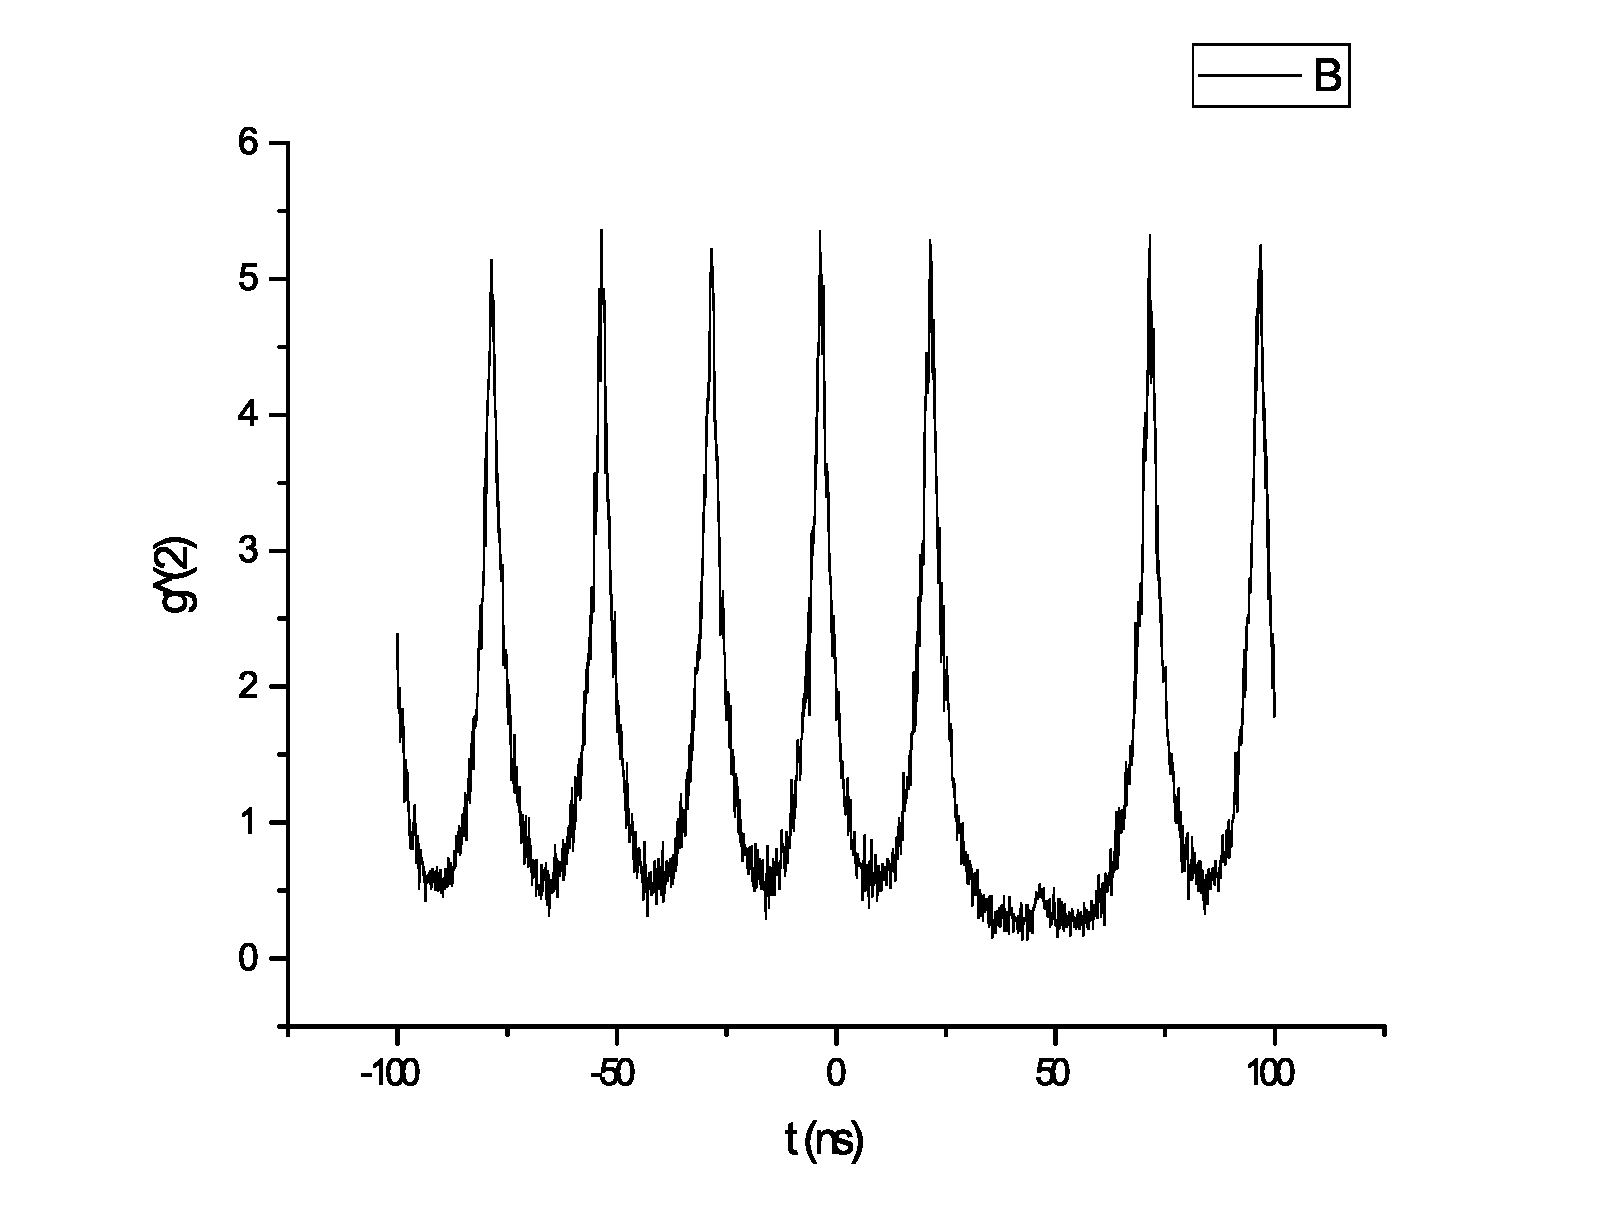
\includegraphics[trim = 0 0 0 0,  clip= true, width = \textwidth]{./pics/siv_sarah_g2_2.pdf}}
			\label{subfig::erlangen_g2_pulsed}
		\end{subfigure}
		\caption{\gtz measurements of emitter \correct{xx} a) power-dependent, continuous excitation, b) pulsed excitation}
		\label{fig::erlangen_g2}
	\end{figure}

	\begin{figure}[tp]
		\begin{subfigure}[t]{ 0.49\linewidth}
			\centering
			\testbox{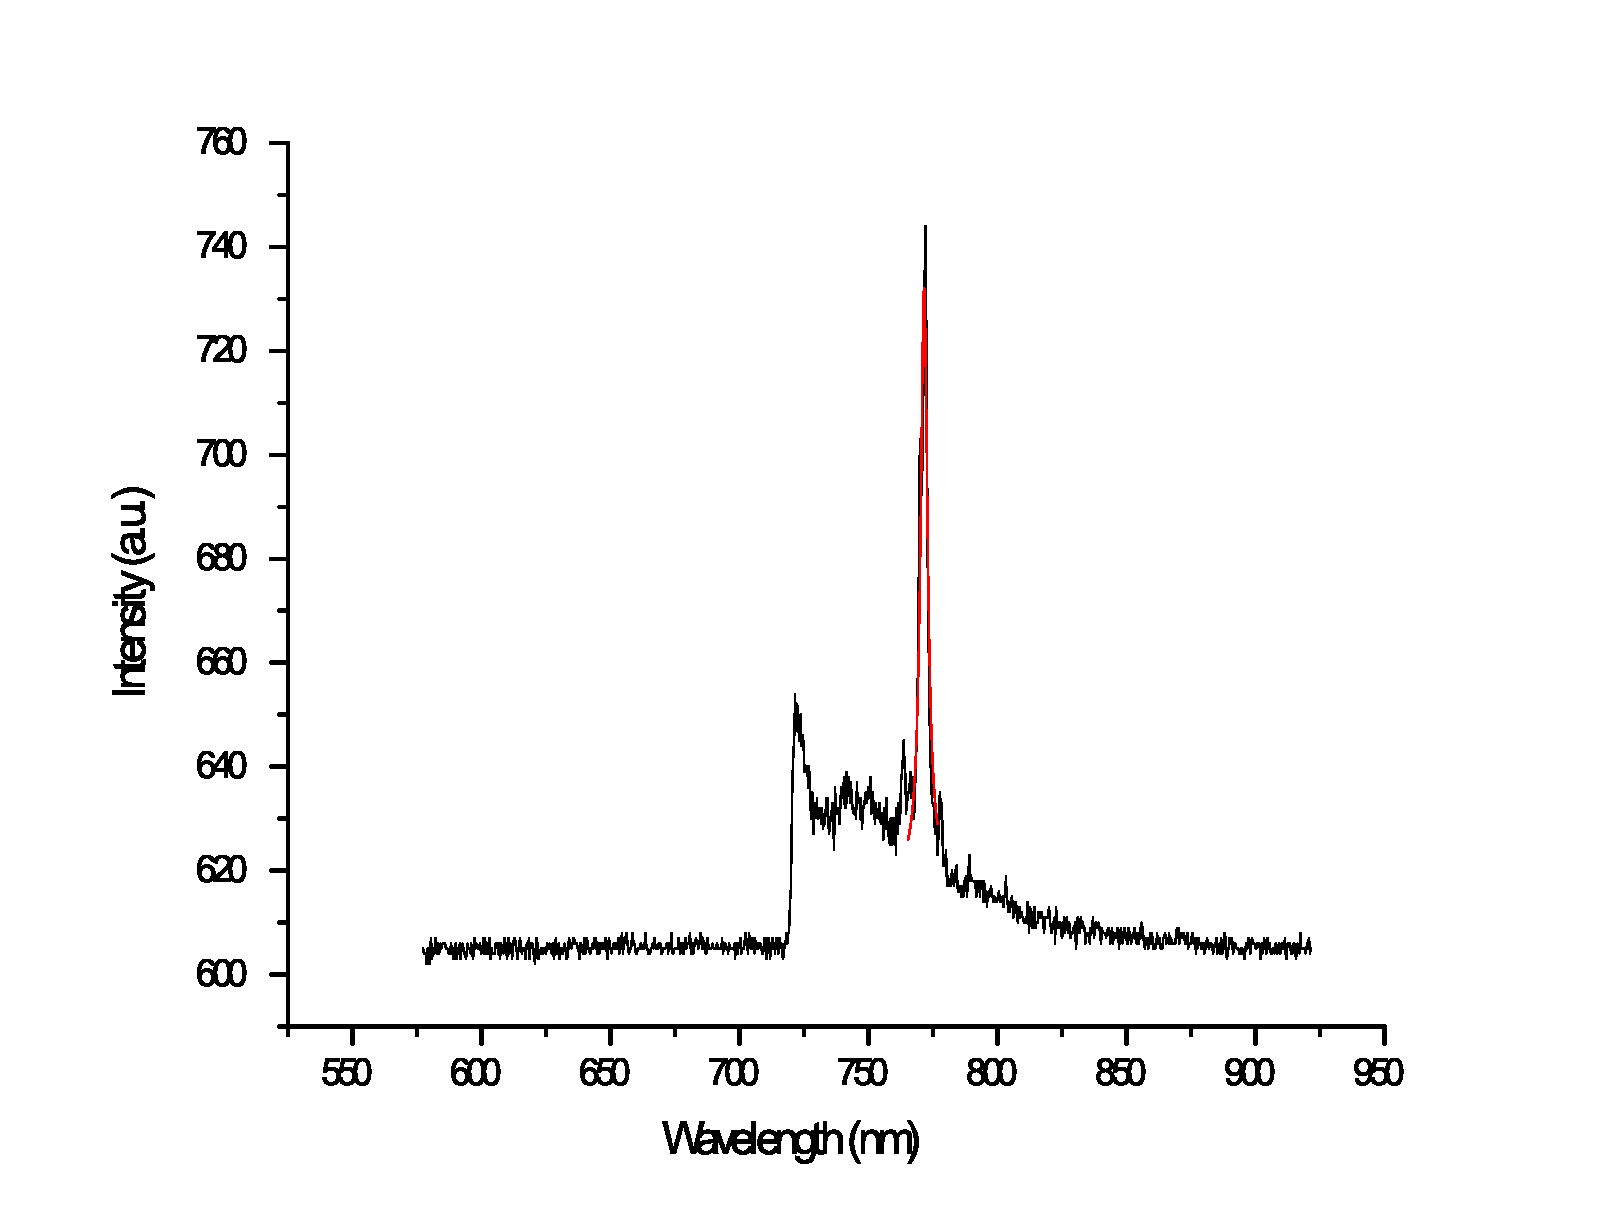
\includegraphics[trim = 0 0 0 0,  clip= true, width = \textwidth]{./pics/Siv_sarah_spectra2_1.pdf}}
			\caption{}
			\label{subfig::erlangen_spectrum}
		\end{subfigure}
		\hfill
		\begin{subfigure}[t]{ 0.49\linewidth}
			\centering
			\testbox{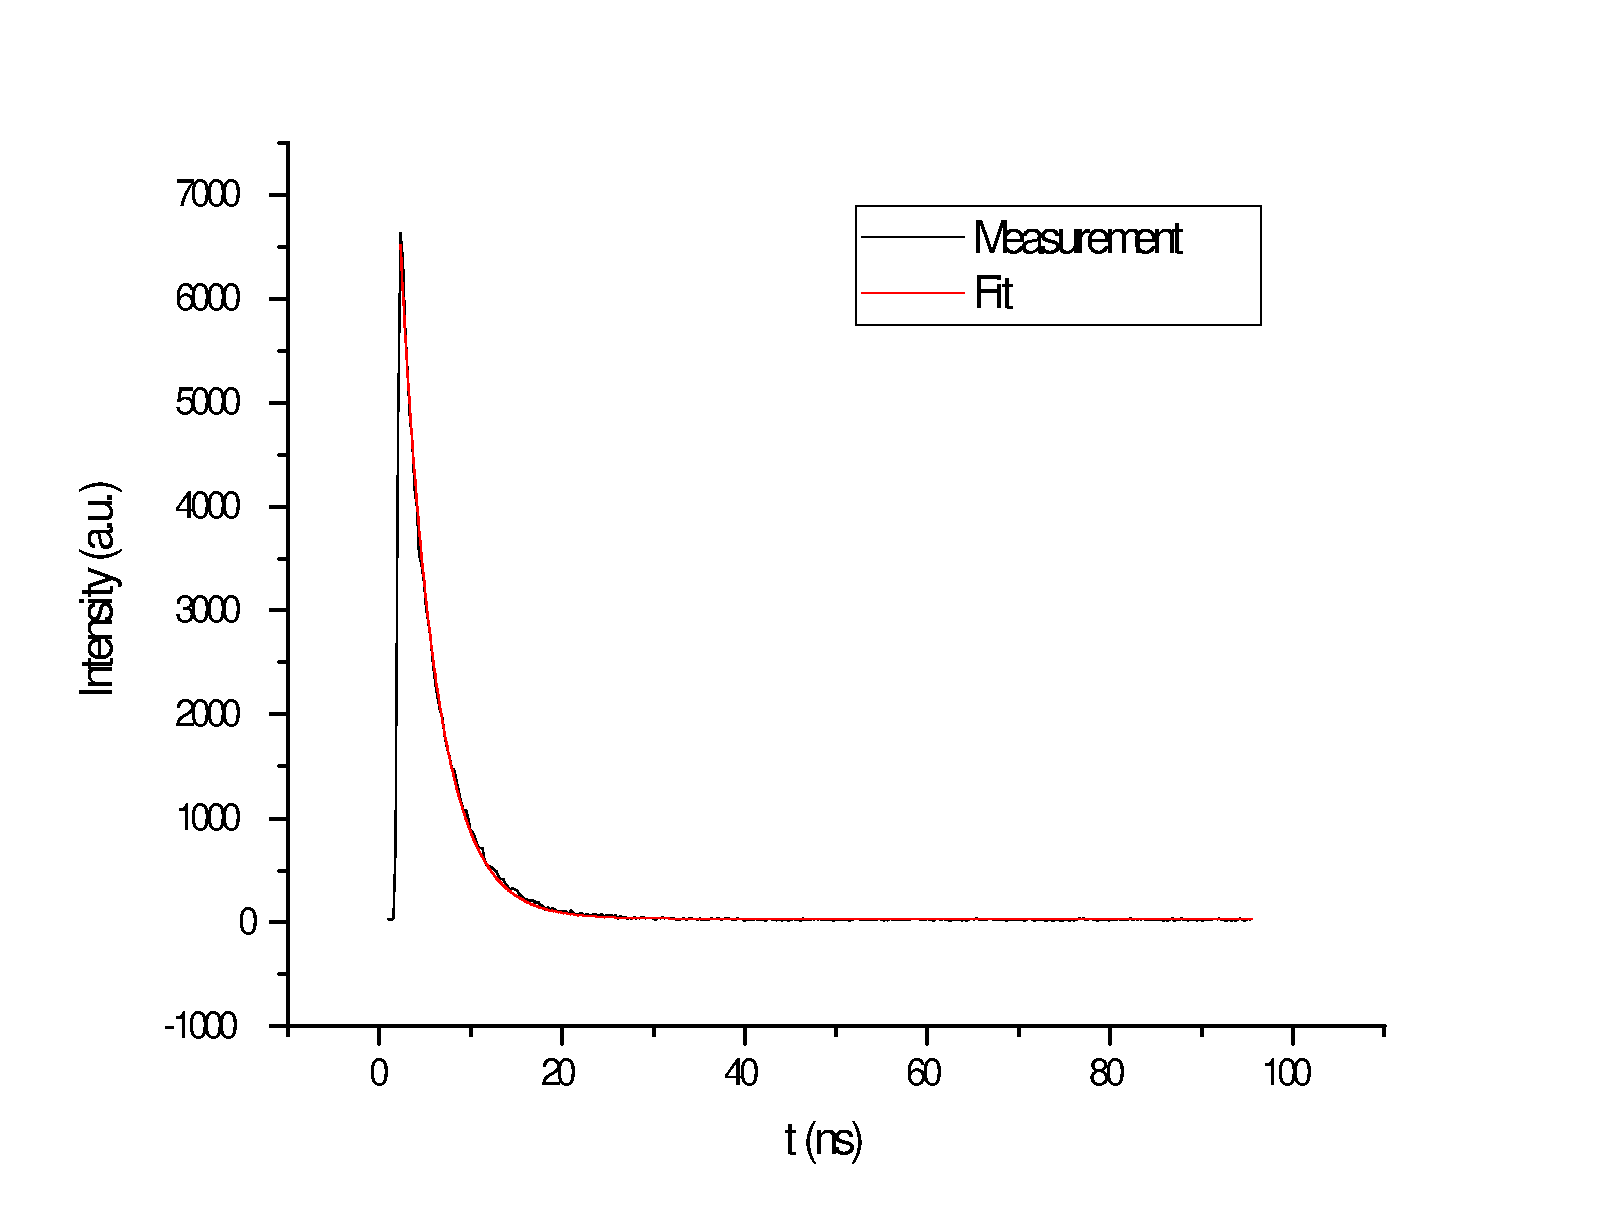
\includegraphics[trim = 0 0 0 0,  clip= true, width = \textwidth]{./pics/siv_sarah_lifetime_2.pdf}}
			\caption{}
			\label{subfig::erlangen_lifetime}
		\end{subfigure}
		\caption{a) Spectrum of emitter \correct{xx} b) lifetime measurement of emitter \correct{xx}}
		\label{fig::erlangen_spectrum_lifetime}
	\end{figure}

